\documentclass[11pt]{article}
%\documentclass[12pt]{article}
%\documentclass[12pt,a4paper]{article}

\usepackage[percent]{overpic}
\usepackage{float}
\usepackage{makecell}
\usepackage{pgfplots}
%\usepackage[cmbold]{mathtime}
%\usepackage{mt11p}
\usepackage{placeins}
\usepackage{amsmath}
\usepackage{amsthm}
\usepackage{color}
\usepackage{amssymb}
\usepackage{mathtools}
\usepackage{subfigure}
\usepackage{multirow}
\usepackage{epsfig}
\usepackage{listings}
\usepackage{enumitem}
\usepackage{rotating,tabularx}
%\usepackage[graphicx]{realboxes}
\usepackage{graphicx}
\usepackage{graphics}
\usepackage{epstopdf}
\usepackage{longtable}
\usepackage[pdftex]{hyperref}
%\usepackage{breakurl}
\usepackage{epigraph}
\usepackage{xspace}
\usepackage{amsfonts}
\usepackage{eurosym}
\usepackage{ulem}
\usepackage{footmisc}
\usepackage{comment}
\usepackage{setspace}
\usepackage{geometry}
\usepackage{caption}
\usepackage{pdflscape}
\usepackage{array}
\usepackage[round]{natbib}
\usepackage{booktabs}
\usepackage{dcolumn}
\usepackage{mathrsfs}
%\usepackage[justification=centering]{caption}
%\captionsetup[table]{format=plain,labelformat=simple,labelsep=period,singlelinecheck=true}%

%\bibliographystyle{unsrtnat}
\bibliographystyle{ecta}
\usepackage{enumitem}
\usepackage{tikz}
\usetikzlibrary{decorations.pathreplacing}
%\def\checkmark{\tikz\fill[scale=0.4](0,.35) -- (.25,0) -- (1,.7) -- (.25,.15) -- cycle;}
%\usepackage{tikz}
%\usetikzlibrary{snakes}
%\usetikzlibrary{patterns}

%\draftSpacing{1.5}

\usepackage{xcolor}
\hypersetup{
colorlinks,
linkcolor={blue!50!black},
citecolor={blue!50!black},
urlcolor={blue!50!black}}

%\renewcommand{\familydefault}{\sfdefault}
%\usepackage{helvet}
%\setlength{\parindent}{0.4cm}
%\setlength{\parindent}{2em}
%\setlength{\parskip}{1em}

%\normalem

%\doublespacing
\onehalfspacing
%\singlespacing
%\linespread{1.5}

\newtheorem{theorem}{Theorem}
\newcommand{\bc}{\begin{center}}
\newcommand{\ec}{\end{center}}
\newtheorem{corollary}[theorem]{Corollary}
\newtheorem{proposition}{Proposition}
\newtheorem{definition}{Definition}
\newtheorem{axiom}{Axiom}
\newcommand{\ra}[1]{\renewcommand{\arraystretch}{#1}}

\newcommand{\E}{\mathrm{E}}
\newcommand{\Var}{\mathrm{Var}}
\newcommand{\Corr}{\mathrm{Corr}}
\newcommand{\Cov}{\mathrm{Cov}}

\newcolumntype{d}[1]{D{.}{.}{#1}} % "decimal" column type
\renewcommand{\ast}{{}^{\textstyle *}} % for raised "asterisks"

\newtheorem{hyp}{Hypothesis}
\newtheorem{subhyp}{Hypothesis}[hyp]
\renewcommand{\thesubhyp}{\thehyp\alph{subhyp}}

\newcommand{\red}[1]{\textcolor{red} {#1}}
\newcommand{\blue}[1]{\textcolor{blue} {#1}}
\newcommand{\green}[1]{\textcolor{green}{#1}}

%\newcommand*{\qed}{\hfill\ensuremath{\blacksquare}}%

\newcolumntype{L}[1]{>{\raggedright\let\newline\\arraybackslash\hspace{0pt}}m{#1}}
\newcolumntype{C}[1]{>{\centering\let\newline\\arraybackslash\hspace{0pt}}m{#1}}
\newcolumntype{R}[1]{>{\raggedleft\let\newline\\arraybackslash\hspace{0pt}}m{#1}}

%\geometry{left=1.25in,right=1.25in,top=1.25in,bottom=1.25in}
\geometry{left=1in,right=1in,top=1in,bottom=1in}

\epstopdfsetup{outdir=./}

\newcommand{\elabel}[1]{\label{eq:#1}}
\newcommand{\eref}[1]{Eq.~(\ref{eq:#1})}
\newcommand{\ceref}[2]{(\ref{eq:#1}#2)}
\newcommand{\Eref}[1]{Equation~(\ref{eq:#1})}
\newcommand{\erefs}[2]{Eqs.~(\ref{eq:#1}--\ref{eq:#2})}

\newcommand{\Sref}[1]{Section~\ref{sec:#1}}
\newcommand{\sref}[1]{Sec.~\ref{sec:#1}}

\newcommand{\Pref}[1]{Proposition~\ref{prop:#1}}
\newcommand{\pref}[1]{Prop.~\ref{prop:#1}}
\newcommand{\preflong}[1]{proposition~\ref{prop:#1}}

\newcommand{\Aref}[1]{Axiom~\ref{ax:#1}}
\newcommand{\Dref}[1]{Definition~\ref{def:#1}}

\newcommand{\clabel}[1]{\label{coro:#1}}
\newcommand{\Cref}[1]{Corollary~\ref{coro:#1}}
\newcommand{\cref}[1]{Cor.~\ref{coro:#1}}
\newcommand{\creflong}[1]{corollary~\ref{coro:#1}}

\newcommand{\etal}{{\it et~al.}\xspace}
\newcommand{\ie}{{\it i.e.}\xspace}
\newcommand{\eg}{{\it e.g.}\xspace}
\newcommand{\etc}{{\it etc.}\xspace}
\newcommand{\cf}{{\it c.f.}\xspace}
\newcommand{\ave}[1]{\left\langle#1 \right\rangle}
\newcommand{\person}[1]{{\it \sc #1}}

\newcommand{\AAA}[1]{\red{{\it AA: #1 AA}}}
\newcommand{\YB}[1]{\blue{{\it YB: #1 YB}}}

\newcommand{\flabel}[1]{\label{fig:#1}}
\newcommand{\fref}[1]{Fig.~\ref{fig:#1}}
\newcommand{\Fref}[1]{Figure~\ref{fig:#1}}

\newcommand{\tlabel}[1]{\label{tab:#1}}
\newcommand{\tref}[1]{Tab.~\ref{tab:#1}}
\newcommand{\Tref}[1]{Table~\ref{tab:#1}}

\newcommand{\be}{\begin{equation}}
\newcommand{\ee}{\end{equation}}
\newcommand{\bea}{\begin{eqnarray}}
\newcommand{\eea}{\end{eqnarray}}

\newcommand{\bi}{\begin{itemize}}
\newcommand{\ei}{\end{itemize}}

\newcommand{\Epsilon}{\mathcal{E}}
\newcommand{\etau}{\tau^\text{eqm}}
\newcommand{\wtau}{\widetilde{\tau}}
\newcommand{\xN}{\ave{x}_N}
\newcommand{\Sdata}{S^{\text{data}}}
\newcommand{\Smodel}{S^{\text{model}}}

\newcommand{\del}{D}
\newcommand{\hor}{H}
\newcommand{\subhead}[1]{\mbox{}\newline\textbf{#1}\newline}
\newcommand{\ND}{\mathcal{N}} % Normal Distribution
\newcommand{\sigman}[1]{{\sigma^{(#1)}}}
\newcommand{\sigmat}{\tilde{\sigma}}
\newcommand{\sigmac}{{\sigma_\rho}}
\newcommand{\var}[1]{\text{var}(#1)}


\newcommand{\ve}{\ensuremath{\varepsilon}\xspace}								
\newcommand{\mh}{\ensuremath{\hat{\mu}}\xspace}
\newcommand{\Du}{\ensuremath{\Delta u}\xspace}
\newcommand{\Dx}{\ensuremath{\Delta x}\xspace}
\newcommand{\dx}{\ensuremath{\delta x}\xspace}
\newcommand{\Dt}{\ensuremath{\Delta t}\xspace}
\newcommand{\dt}{\ensuremath{\delta t}\xspace}
\newcommand{\dW}{\ensuremath{\dif W}\xspace}


\newcommand{\EV}[1]{\ensuremath{\operatorname{E}\left[ #1 \right]}\xspace}	% Exp. Value Operator
\newcommand{\V}[1]{\ensuremath{\operatorname{Var}\left[ #1 \right]}\xspace}	% Variance Operator
\newcommand{\EA}[1]{\ensuremath{\left\langle#1\right\rangle}\xspace}		% ensemble averageof #1
\newcommand{\TA}[1]{\ensuremath{\bar{#1}}\xspace}											% Time average of #1
\newcommand{\muest}{\hat{\mu}}
\newcommand{\sm}{\sigma_\mu}
\newcommand{\lev}{\ensuremath{\ell}\xspace}
\newcommand{\lo}{\ensuremath{\lev_{\text{opt}}}\xspace}							% optimal leverage
\newcommand{\lou}{\ensuremath{\lev_{\text{opt}}^*}\xspace}% optimal leverage of the perturbed gamble
\newcommand{\lob}{\ensuremath{{\lev^b_{\text{opt}}}}\xspace}				% optimal leverage dependent on b 
\newcommand{\lobu}{\ensuremath{\lev^{b*}_{\text{opt}}}\xspace}		% uncertainty adjusted optimal

\newcommand{\EE}{\textit{Ergodicity Economics}\xspace}
\newcommand{\BD}{\mathcal{B}} % Bernoulli/Binomial Distribution

\newcommand{\LND}{\mathcal{L}} % LogNormal Distribution

\newcommand{\NN}{\ensuremath{\mathbb{N}}\xspace} 		% set of natural numbers

\newcommand{\tq}[1]{\textquote{#1}}

\setlength{\parindent}{0.0cm}
\setlength{\parskip}{0.4em}

\numberwithin{equation}{section}
\DeclareMathOperator\erf{erf}
%\let\endtitlepage\relax

\begin{document}

%\onehalfspacing
\begin{titlepage}
%\title{Temporal Discounting Without Uncertainty: Growth Rates, Preference Reversal and Hyperbolic Discounting}
\title{Probability weighting as model calibration}
\author{Ole Peters\footnote{London Mathematical Laboratory and Santa Fe Institute,~\url{o.peters@lml.org.uk}}  \and Alexander Adamou\footnote{London Mathematical Laboratory,~\url{a.adamou@lml.org.uk}} \and Mark Kirstein\footnote{London Mathematical Laboratory,~\url{m.kirstein@lml.org.uk}}  \and Yonatan Berman\footnote{London Mathematical Laboratory,~\url{y.berman@lml.org.uk}} \,\, %\thanks{}
}
%\date{First version: August 26, 2018\,\,\,\,\,\,\,\,\,\,\,\,\,\,\,\,\,\,\,\,\,\,\,\,Last revised: \today}
%\date{}
\date{\today}
\maketitle

%\bc
%\red{Preliminary version, please do not circulate}
%\ec

\begin{abstract}
\noindent 
Behavioral economics collects observations of human economic behavior and provides labels for those observations. 
Probability weighting is one such label. It expresses a mismatch, in decision problems, between probabilities used in a formal model of a decision problem (\ie model parameters) and probabilities inferred from real people's behavior faced with the modelled decision problem (the same parameters estimated empirically). The inferred probabilities are called ``decision weights.'' 
It is considered a robust observation that decision weights are higher than probabilities for extreme events, and (necessarily, because of normalization) lower than probabilities for common events.
The observed behavior thus amounts to the refusal by real decision-makers totally to rely on a formal model, and instead to exercise extra caution. In this paper we model well-specified reasons for such caution and find the resulting probability weighting, as a benchmark for reasonable behavior. We find close agreement with empirical studies.
\\
\\


\noindent\textbf{Keywords: decision theory, prospect theory, probability weighting, ergodicity economics}
%\\
%\noindent\textbf{JEL codes: D8, D9}\\

%\bigskip
\end{abstract}
\setcounter{page}{0}
\thispagestyle{empty}
%\nopagebreak
\end{titlepage}
\pagebreak \newpage
%\nopagebreak

\section{Introduction and outline}
Probability weighting originates in prospect theory  \citep{Barberis2013}. It is one way to conceptualize a pattern in human behavior of caution with respect to formal models. This is best explained with an example: a decision maker (DM) is told by a disinterested observer (DO), such as an experimenter, that an event occurs with some probability. The DM's behaviour is then observed, and is found to be consistent with a behavioural model (for example expected-utility optimization) where the DM uses a probability that differs systematically from what the DO has declared. 

Specifically, it is consistently observed that DMs act as though extreme events (those of low probability) had higher probabilities than what's specified by the DO. These apparent ``higher probabilities'' are called ``decision weights'' because they are better at describing the decisions actually made than the probabilities specified by the DO. We will adopt this nomenclature here. By ``probabilities,'' denoted $p$, we will mean the numbers specified by a DO, and by ``decision weights,'' denoted $w$, we will mean the numbers that best describe the behaviour of a DM.\footnote{In the literature, decision weights are not always normalised, but for simplicity we will work with normalised decision weights. Mathematically speaking, they are therefore proper probabilities even though we don't call them that. Our results are unaffected because normalizing just means dividing by a constant (the sum or integral of the non-normalised decision weights).}

We will show below that these observations are predicted by considerations of uncertainty about probabilities, or more generally by uncertainty about model parameters. 

We begin by discussing the necessity for using decision weights that are greater than the probabilities for rare events. Next, we discuss as an example how the same effect can arise when repeatedly facing prospects with a Gaussian random variable whose mean fluctuates in time.

Finally, we calculate analytically, and plot, the probability weighting curves one would expect on this basis. We compare these to the empirical results summarised by \citet{Barberis2013}, and we comment on the function fitted to these data by \citet{TverskyKahneman1992}.

Our work contributes to the growing field of ergodicity economics
\citep{Peters2019b} where decision makers are modelled as behaving optimally over time (as opposed to optimally in a statistical-ensemble sense).

\section{Consistent probability weighting as a difference between models}
We will put forward the possibility that probability weighting as observed in studies related to prospect theory is a mismatch between models of the world, specifically between probabilities assigned to events in models of the world. For this to be a likely explanation of the phenomenon, two conditions must be satisfied. First, there must be a reason for common disagreement in how probabilities are modelled; second, there must be a reason for such disagreement to be consistent: there must be a relevant systematic difference between the modeller or scientist (DO) on the one hand, and the test subject or actor in the real world (DM) on the other hand. 

The first condition is satisfied because the word ``probability'' is commonly interpreted in different ways. Even once one has settled on a definition, numerical values for probabilities are still difficult to estimate from real-world observations.

The second condition is satisfied as follows. A DO has systematically different incentives from a real-world DM. The DO tends to have an incentive to estimate, or indeed state, probabilities as their most likely value or ``true'' value (if the DO can control the probabilities, \eg in an experiment); the DM simply strives to behave optimally under uncertainty, and that uncertainty often includes uncertainty about the probabilities or model parameters.

\subsection{Probabilities are tricky}
\subhead{Lack of conceptual clarity}
It's not easy to unpack a simple probability statement like ``the probability of rain here tomorrow is 70\%.'' Tomorrow only happens once, so rain happens in 70\% of what? The technical answer to this question is usually: rain happens in 70\% of the members of an ensemble of computer-simulations, run by a weather service, of what may happen tomorrow. So one interpretation of ``probability'' is ``relative frequency in a hypothetical ensemble of possible futures.'' 

How exactly such a statement is linked to physical reality is not completely clear. Sometimes ensembles are real, for instance, when we say the probability of having a car accident is 1\% per 10,000km driven -- that's a summary of statistics collected over a large ensemble of cars. In this case, it's a real ensemble that existed in the past, not an imagined one in the future. 

In some situations, the statement 70\% chance of rain tomorrow refers to the relative frequency over time. Before the advent of computer models in weather forecasting, people used to compare recent measurements (of wind and pressure today, say) to measurements further in the past - weeks, months, years earlier, that were similar and where one had reason to believe that what had happened 1 day later would be similar to what will happen tomorrow.

No matter how ``probability'' relates to a frequentist physical statement (whether with respect to an ensemble of simultaneous possibilities or to a time series), it also corresponds to a mental state of believing something with a degree of conviction: ``I'm 90\% sure I left my wallet in that taxi.''

Many long books have been written about the meaning of probability; for our purpose it suffices to say that there's no guarantee that a probabilistic statement will be interpreted by the listener as it was intended by whoever made the statement.

\subhead{Estimation errors for probabilities}
Finally, let's imagine the DO and DM have agreed explicitly on an interpretation of the word ``probability.'' Say they agree that they mean the relative frequency in a long time series. Real time series are, of course, of finite length. In order to estimate the relative frequency of some event in a time series, we basically count -- out of $T$ time intervals, the event $i$ occurred in $n_i$ of them, so our best estimate for the probability is $n_i/T$. In the simplest case (and we rarely consider anything more complicated), we model the arrival of events as a Poisson process, where the standard error in the count of an event famously goes as $\sqrt{n_i}$. The standard error in the probability of an event is therefore $\frac{\sqrt{n_i}}{T}$, and the relative error is $\frac{1}{\sqrt{n_i}}$. Low probabilities therefore come with larger relative errors, see \tref{errors}. We note that behaviourally, it will make little difference whether a DM assigns a 0.49 probability to an event or a 0.51 probability. It will make a large difference, however, whether a DM assigns a 0 probability or a 0.0002 probability.
The most important message from this example computation is that errors in probability estimates behave differently for small probabilities than for large probabilities: absolute errors are smaller for small probabilities, and relative errors are larger for small probabilities.

\begin{table}[!htb]
\ra{1.25}
%\small
\centering
\captionof{table}{This table assumes $T=$10,000 observed time intervals. To be read as follows (first line): for an event of true probability 0.5, the most likely count in 10,000 trials is 5,000. Assuming Poissonian statistics, this comes with an estimation error of $\sqrt{5,000}/10,000=0.01$, which is 2\% of the true probability.}\tlabel{errors}
\begin{tabular}{@{}cccc@{}}\toprule[2pt]
\makecell{Asymptotic\\(true) probability} & \makecell{Most likely\\count} & \makecell{Estimation\\error} & \makecell{Relative\\error}\\
\midrule[2pt]
.5 & 5000 & .01 & 2\%\\
.1 & 1000& .003 & 3\%\\
.01 & 100& .001 & 10\%\\
.001 & 10& .0003& 30\%\\
.0001 & 1& .0001 &100\%\\
\bottomrule[2pt]
\end{tabular}
\end{table}

\subsection{Disinterested observers and decision makers have different incentives}
The observations that led to the concept of probability weighting in prospect theory can be expressed as follows: DOs assign systematically lower weights to low-probability events than DMs.
Crucially, which of the two is wrong is unclear so long as it is unclear who means what by the word ``probability.'' Because the two types of modellers (DO and DM) pursue different goals, it may be the case that neither is wrong about the probabilities, just wrong about the goals of the other modeller.

Being a good neutral scientist, a DO has no particular interest in the success or failure of a DM. Being a good DM, the DM has every interest in the success or failure of the DM. Throughout the history of economics, it has been a common mistake, by DOs, to assume that DMs optimise what happens to them on average in an ensemble. To the DM what happens to the ensemble is usually not a primary concern -- instead, the concern of the DM is what happens to him over time. Not distinguishing between these two perspectives is only permissible if they lead to identical predictions, and that is only the case in ergodic situations \citep{Peters2019b}. 

It is now well known that the situation usually studied in decision theory is not ergodic in the following sense: DMs are usually observed making choices that affect their wealth, and wealth is usually modelled as a stochastic process that is not ergodic. The ensemble average of wealth does not behave like the time average of wealth.

The most striking example is the universally important case of noisy multiplicative growth -- universal because it is the fundamental process that drives evolution: noise generates the diversity (of phenotypes) necessary for evolution, and multiplicative growth (self-reproduction) is how successful phenotypes spread their traits in a population. This process operates on amoeba, as it does on forms of institutions, and on investment strategies. 

The simplest model of noisy multiplicative growth is geometric Brownian motion, $dx=x(\mu dt+\sigma dW)$. The average over the full statistical ensemble (often studied by the DO) of geometric Brownian motion grows as $\exp(\mu t)$. The individual trajectory of geometric Brownian motion, on the other hand, grows in the long run as $\exp[(\mu-\frac{\sigma^2}{2})t]$.

In the DO's ensemble perspective, noise does not affect growth and is often deemed irrelevant.

In the DM's time perspective, noise reduces growth, and {\it underestimating it would have catastrophic consequences.}

The difference between how these two perspectives evaluate the effects of noise (\ie of the probabilistic events) is qualitatively in line with the observed phenomena we set out to explain. The DM typically has large uncertainties, especially for small-probability events, and has an evolutionary incentive to err on the side of caution, \ie to behave as though low-probability (extreme) events had a higher probability.

It remains to quantify these considerations and work through a key example.

\section{The Gaussian case}
%A systematic bias for decision weights to be higher than probabilities for low-probability events is a basic rule for survival. Extreme events (those of low probability) have two important properties. First, they're rare by definition; second, they're the most disruptive events. 
%
%These two facts have two consequences: first, the rarity implies that in a model fitted to observations, we will have poor statistics for such events and large uncertainty about their frequency (or ``probability''); second, because they're disruptive we have to make sure we're well prepared for them. These two facts translate into the survival rule: bias your estimates of frequencies of extreme events to be high. 
%
%To illustrate the spirit of this thought: if we think a category-5 hurricane hits once every 50-100 years, and we have to make provisions of some sort to ensure we can recover from such an event, then we have to assume the higher frequency in order to be properly prepared, \ie we have to assume the event will hit with a frequency of 1/50 p.a. Using a central value, like 1/75 p.a. would be unwise.
We have so far established that evolution forces DMs to estimate the magnitude of noise cautiously, meaning: to err on the high side.
As a concrete fully quantitative formal example, let's say the annual logarithmic returns, $g$, on our pension portfolio are Gaussian-distributed (yes, that may be a bad model). Let's also say we have some observations and estimate the variance of these returns to be $\sigma_1^2 \pm \sigma_2^2$. A DO without exposure to these returns would quite reasonably model them with a central best-estimate variance as $g_p \sim \ND(\mu, \sigma_1^2)$.

A DM, on the other hand, would want to be on the safe side, and would assume the upper end of the range that's considered plausible for the variance. The DM would use the model $g_w \sim \ND(\mu, \sigma_1^2+\sigma_2^2$). Because the variance of the decision weights is higher than the variance of the probabilities, the decision weight corresponding to an extreme event will be higher than its probability, see \fref{probability_dists}.

\begin{figure}[!htb]
\centering
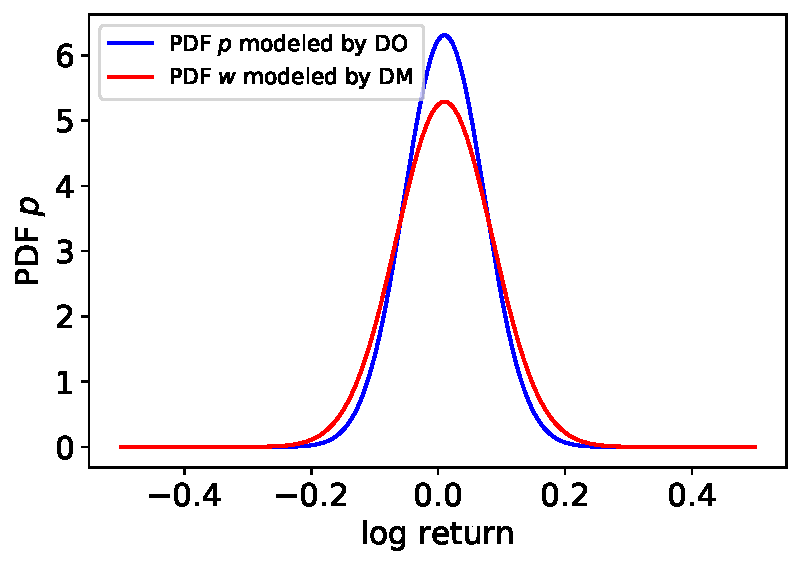
\includegraphics[width=0.7\textwidth]{./figs/probability_dists.pdf}
\caption{Probability density function (blue), estimated by a DO; and decision-weight density function (red), estimated by a DM. The DO models returns with a best estimate for the variance and assumes the true frequency distribution is the blue line. The DM wants to be on the safe side, models returns with a greater variance, and assumes the true frequency distribution is the red line. The DM appears to the DO as someone who over-estimates probabilities of low-probability events and underestimates probabilities of high-probability events.}
\flabel{probability_dists}
\end{figure}

%
%\subsection{Repetition and location uncertainty}
%
%Let's stay with the investment example, and again say annual logarithmic returns are Gaussian-distributed. Let's also assume (somewhat unrealistically) that we know the variance of these returns to be $\sigma_1^2$, with certainty.
%
%Finally, we assume that the mean of the returns fluctuates. Over time, we don't always draw from the same Gaussian, but sometimes from one with a larger mean and sometimes from one with a smaller mean.
%We implement this as follows: first, generate a mean, $\gamma$, from a Gaussian distribution $\gamma \sim \ND(\mu, \sigma_2^2)$. Then draw a return from a Gaussian with this mean and variance $\sigma_1^2$, meaning $g\sim\ND(\gamma,\sigma_1^2)$. Over time, the total log return is just the sum of the annual log returns, and it is equivalent to the total log return that would be generated with a Gaussian with known mean and higher variance, $g\sim \ND(\mu,\sigma_1^2+\sigma_2^2)$.
%
%Considering a single round, a DO might well use the best estimate for $\gamma$, which is $\mu$, and the known variance $\sigma_1^2$, so that $g_p\sim \ND(\mu,\sigma_1^2)$. A DM, on the other hand, who has to live with the consequences of what happens in a long sequence realizations of $g$ would use $g_w\sim \ND(\mu,\sigma_1^2+\sigma_2^2)$. Again, the situations and incentives of the DO and the DM are different, leading them to use different models (the same models as in \Secref{Survival})
%
%\section{Analysis of the Gaussian case}
%The point of the previous two sub-sections was to illustrate two different ways in which uncertainty or fluctuations in parameters lead to behaviour by a DM that leads to greater decision weights for extreme events than the probabilities a DO might assign to them. In the first case, the DO uses the best estimate, rather than a conservative estimate of the variance. In the second case, the DO assumes no fluctuations in the mean return.
%
%Both DO models give $g_p\sim\ND(\mu,\sigma_1^2)$, whereas the DM will choose the model $g_w \sim \ND(\mu,\sigma_1^2+\sigma_2^2)$.

The effect of the DM using a higher variance in his model is an over-estimate of low-probability events. Because of normalization, overestimating low probability events necessarily implies underestimating high-probability events, see \fref{probability_dists}.

We can choose to express the DM's behaviour in terms of a mapping between the decision weights used by the DM, $w$ (red in \fref{probability_dists}), and the probabilities estimated by the DO, $p$ (blue in \fref{probability_dists}).

In the Gaussian case we can write the distributions explicitly
\be
w=\frac{1}{\sqrt{2\pi (\sigma_1^2+\sigma_2^2)}}\exp\left[\frac{-(g -\mu )^2}{2 (\sigma_1^2+\sigma_2^2)}\right]
\elabel{q}
\ee
and
\be
p=\frac{1}{\sqrt{2\pi \sigma_1^2}}\exp\left[\frac{-(g -\mu )^2}{2 \sigma_1^2}\right].
\elabel{p}
\ee

Furthermore, we can solve \eref{p} for $(g -\mu )^2$ and substitute that in in \eref{q}. Thereby, we obtain the following expression for decision weights directly as a function of probabilities
\be
w(p)=p^{\frac{\sigma_1^2}{\sigma_1^2+\sigma_2^2}} \frac{\left(\sqrt{2\pi\sigma_1^2}\right)^{\frac{\sigma_2^2}{\sigma_1^2+\sigma_2^2}}}{\sqrt{2\pi(\sigma_1^2+\sigma_2^2)}},
\elabel{q_of_p}
\ee
which we plot in \fref{probability_weights}. 

\begin{figure}[!htb]
\centering
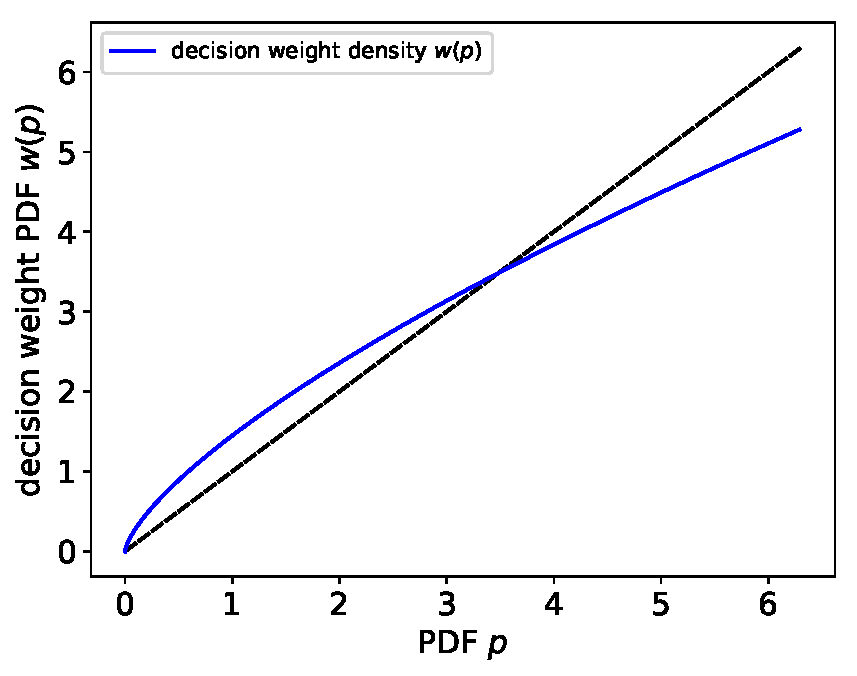
\includegraphics[width=0.7\textwidth]{./figs/decision_weights.pdf}
\caption{Decision weight density (used by a DM) vs. probability density (used by a DO) for the Gaussian model (blue), compared to the diagonal (black) where DM and DO use the same parameters. For low probabilities, the decision weights are higher than the probabilities; for high probabilities they are lower.}
\flabel{probability_weights}
\end{figure}

In discussions of probability weighting, it is common to plot cumulative density functions (CDFs) for decision weights versus CDFs for probabilities. We denote these by $F_p=\int_{-\infty}^x p(s) ds$ (for the DO) and by $F_w=\int_{-\infty}^x w(s) ds$ (for the DM). What happens when $F_w$ is plotted against $F_p$  is illustrated in \fref{decision_map}. We will use the terms scale and location, rather than mean and standard deviation, to emphasise the generality of our arguments: they do not, of course, rely on the Gaussian assumption. 

To clarify this nomenclature: starting with the standard form of a distribution $P(x)$ (of scale 1 and location 0), for example $P_{\text{standard}}(x)\sim \ND(0,1)$, the corresponding distributions of scale $\sigma$ and location $\mu$ are obtained by transforming $x$. With $y=\frac{x-\mu}{\sigma}$, we have $P_{\text{standard}}(y)=\ND(\mu, \sigma^2)$.

\begin{figure}[!htb]
\centering
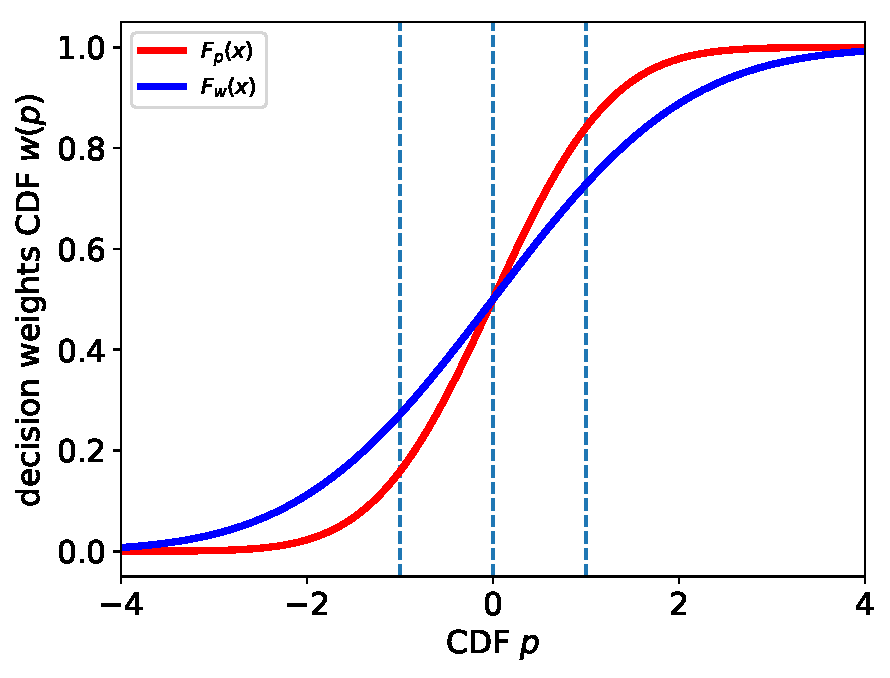
\includegraphics[width=0.7\textwidth]{./figs/decision_map.pdf}
\caption{CDF as assumed by the DO (red) and by the DM (blue), Gaussian distributions, where the DO assumes scale 1 and the DM cautiously assumes scale 2. Following the dashed vertical lines (left to right), we see that for small values of the CDF the DM's is larger than the DO's; the curves coincide at 0.5 because no difference in location is assumed; and for large values of the CDF the DM's is smaller than the DO's }
\flabel{decision_map}
\end{figure}

In \fref{CDF_weights} we show maps that result from the procedure illustrated in \fref{decision_map}. We show separately maps that arise when the DM models the scale of the distribution differently, and when the DM models the location differently. We then put the two together and compare the result to the functional shape \citet{TverskyKahneman1992} chose to fit to their observations.

In \citep{TverskyKahneman1992} cumulative probabilities declared by actual DOs in experiments and decision weights derived from actual DMs' behaviour are compared. Without a mathematical derivation or physical motivation of the functional form, the authors chose to fit the following function to resemble their data
\be
F_{w_{TK}}(F_{p_{TK}})=F_{p_{TK}}^\alpha \frac{1}{(F_{p_{TK}}^\alpha+(1-F_{p_{TK}}))^{1/\alpha}}.
\elabel{correspondence}
\ee

This function 
%resembles the analytical result in that it is essentially a power law in $p_{TK}$, especially if we use $\alpha=\frac{\sigma_1^2}{\sigma_1^2+\sigma_2^2}$. It 
only has one free parameter, $\alpha$, and has the following property: any curvature (\ie any deviation from $F_{w_{TK}}(F_{p_{TK}})=F_{p_{TK}}$, which is the shape it takes for $\alpha=1$) moves the intersection with the diagonal away from the mid-point $1/2$. For this feature to be reproduced it is necessary to introduce a difference between the locations used by DO and DM in addition to the difference between scales. If we allow the possibility that the DM uses different estimates for scale and location, we can reproduce the observations in \citep{TverskyKahneman1992} accurately, see \fref{CDF_weights}.

\begin{figure}
\centering
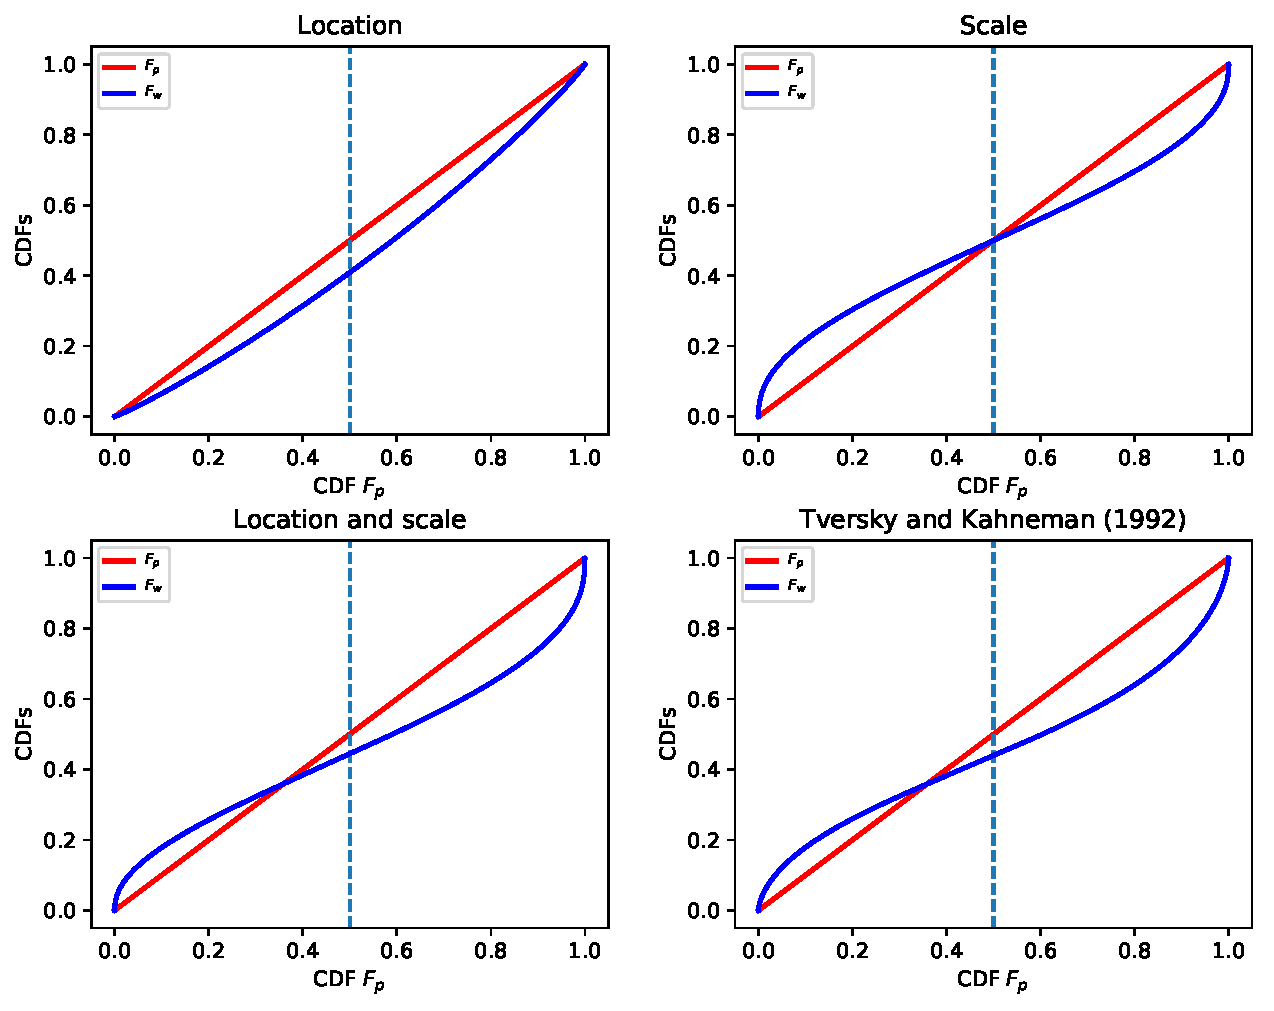
\includegraphics[width=1.0\textwidth]{./figs/Gauss_scale_location_both_KT.pdf}
\caption{Decision weight CDFs used by a DM vs. probability CDFs used by a DO.\\ 
Top left) Gaussian distribution, difference in scale. DO assumes location 0, scale 1; DM assumes location 0, scale 2.7 (broader than DO).\\ 
Top right) Gaussian distribution, difference in location. DO assumes location 0, scale 1; DM assumes location 0.18 (bigger than DO), scale 1.
Bottom left) Gaussian distribution, differences in scale and location. DO assumes location 0, scale 1; DM assumes location 0.18 (bigger than DO), scale 2.7 (broader than DO).\\ 
Bottom right) Fit to observations reported by \citet{TverskyKahneman1992}. This is \eref{correspondence} with $\alpha=0.65$.
The observations by \citet{TverskyKahneman1992} are consistent with a DM assuming a scale and location in real-world decisions that differ from those assumed by the DO.}
\flabel{CDF_weights}
\end{figure}

\section{Other probability distributions}
Numerically, our procedure can be applied to arbitrary distributions: 
\begin{enumerate}
\item
construct a list of values for the CDF assumed by the DO, $F_p(x)$.
\item
construct a list of values for the CDF assumed by the DM, $F_w(x)$.
\item
plot $F_w(x)$ vs $F_p(x)$.
\end{enumerate}
Of course, the DM could assumes a type of distribution that differs from the DO's. An infinity of combinations of assumed distributions can be explored. To illustrate the generality of the procedure, we carry it out for a (power-law tailed) Student-t distribution, \fref{other_CDFs}, where DO and DM use different shape parameters and different locations. The result is qualitatively similar to \fref{CDF_weights} D). 

It is telling that assuming only a difference in scale and location, for the simplest case (Gaussian) reproduces the observations that have come to be known as ``probability weighting.''

\begin{figure}
\centering
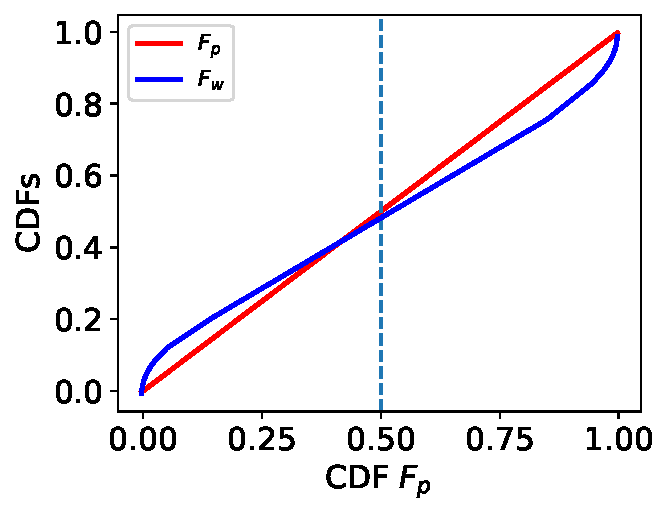
\includegraphics[width=0.7\textwidth]{./figs/Student-t.pdf}
\caption{Probability weighting for Student-t distributions, where the DM uses a different shape parameter (1) and a different location parameter (0) from those of the DO (2 and 0.2, respectively).}
\flabel{other_CDFs}
\end{figure}

\clearpage
%\bibliographystyle{humannat}
\bibliography{./../LML_bibliography/bibliography} % name your BibTeX data base
\end{document}
